\chapter{Results\label{cha:results}}

In the following chapter, the achieved results of the concept are presented. The described approaches are evaluated with regards to the common precision, recall, and F1-Score. Different hyperparameter setups are being discussed and are visualised in graphs. In particular, the baseline approach as described in \ref{glove-approach}, Bert and GPT-2 as described in \ref{transformer-approach} are compared, showing, which vectorisation method yields the best results. Additionally, the regression-based method as described in \ref{sec:regression} and the multi-classification method as described in \ref{sec:classification} are compared, showing advantages or disadvantages among each other.





\section{Experimental Setup}

\subsection{Anomaly Detection on one Dataset}
In order to assess the quality of anomaly detection experiments on one dataset, log alterations, as described in \ref{sec:logs_alteration} are injected with controllable 

\subsection{Transfer Learning}






\section{Evaluation}
\subsection{String cleansing}
String cleansing, as described in \ref{sec:string_cleansing}, drastically improves distinguishability between templates in the used dataset, as depicted in figure \ref{fig:cos_distance_before_cleansing} and figure \ref{fig:cos_distance_after_cleansing} - the templates corresponding to the indices can be found in table \ref{tab:templates_before_cleansing} and table \ref{tab:templates_after_cleansing}, respectively.



\begin{figure}[h]
  \centering
  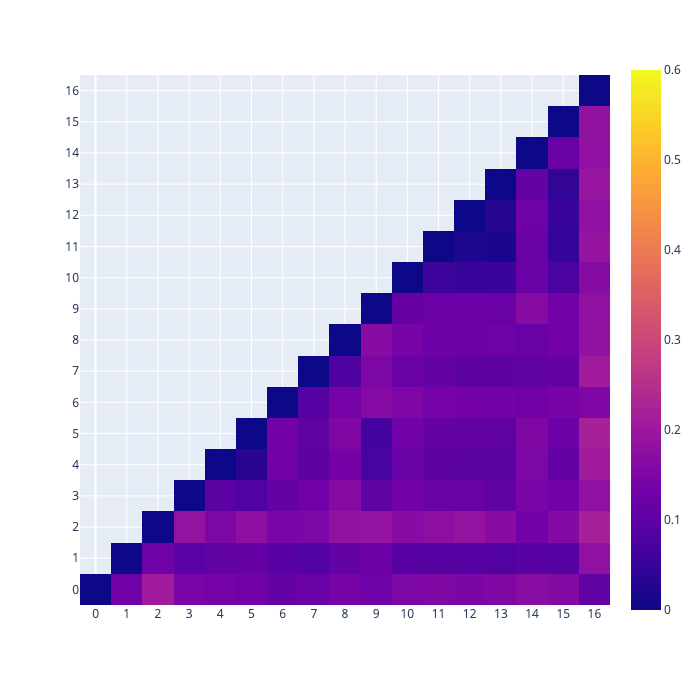
\includegraphics[width=10cm,trim=2cm 2cm .5cm 1cm,clip]{cos_distances_before_clean.png}\\
  \caption{Cosine distance between templates without cleansing}
  \label{fig:cos_distance_before_cleansing}
\end{figure}


\begin{table}[ht]
\begin{small}
\begin{tabular}{ c l } 
\toprule
Index & Template \\
\midrule
0 & $\lang*\rang$ Creating image\\
1 & $\lang*\rang$ VM $\lang*\rang$ (Lifecycle Event)\\
2 & $\lang*\rang$ During sync\_power\_state the instance has a pending task (spawning). Skip.\\
3 & $\lang*\rang$ Instance $\lang*\rang$ successfully.\\
4 & $\lang*\rang$ Took $\lang*\rang$.$\lang*\rang$ seconds to $\lang*\rang$ the instance on the hypervisor.\\
5 & $\lang*\rang$ Took $\lang*\rang$.$\lang*\rang$ seconds to build instance.\\
6 & $\lang*\rang$ Terminating instance\\
7 & $\lang*\rang$ Deleting instance files $\lang*\rang$\\
8 & $\lang*\rang$ Deletion of $\lang*\rang$ complete\\
9 & $\lang*\rang$ Took $\lang*\rang$.$\lang*\rang$ seconds to deallocate network for instance.\\
10 & $\lang*\rang$ Attempting claim: memory $\lang*\rang$ MB, disk $\lang*\rang$ GB, vcpus $\lang*\rang$ CPU\\
11 & $\lang*\rang$ Total memory: $\lang*\rang$ MB, used: $\lang*\rang$.$\lang*\rang$ MB\\
12 & $\lang*\rang$ memory limit: $\lang*\rang$.$\lang*\rang$ MB, free: $\lang*\rang$.$\lang*\rang$ MB\\
13 & $\lang*\rang$ Total disk: $\lang*\rang$ GB, used: $\lang*\rang$.$\lang*\rang$ GB\\
14 & $\lang*\rang$ $\lang*\rang$ limit not specified, defaulting to unlimited\\
15 & $\lang*\rang$ Total vcpu: $\lang*\rang$ VCPU, used: $\lang*\rang$.$\lang*\rang$ VCPU\\
16 & $\lang*\rang$ Claim successful\\
\bottomrule
\end{tabular}
\caption{Templates before cleansing}
\label{tab:templates_before_cleansing}
\end{small}
\end{table}

\begin{figure}[h]
  \centering
  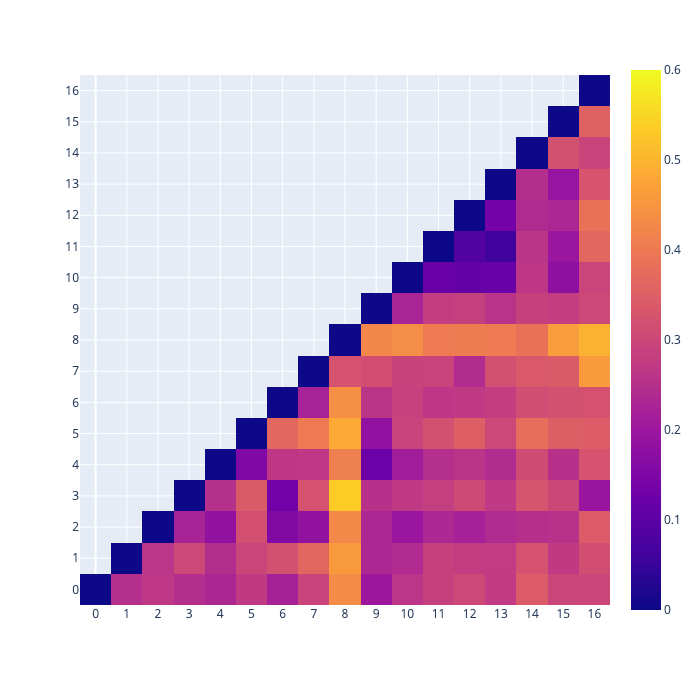
\includegraphics[width=10cm,trim=2cm 2cm .5cm 1cm,clip]{cos_distances_after_clean.png}\\
  \caption{Cosine distance between templates after cleansing}
  \label{fig:cos_distance_after_cleansing}
\end{figure}

\begin{table}[ht]
\begin{small}
\begin{tabular}{ c l } 
\toprule
Index & Template \\
\midrule
0 & Creating image\\
1 & VM  Lifecycle Event\\
2 & During sync power state the instance has a pending task spawning Skip\\
3 & Instance  successfully\\
4 & Took  seconds to  the instance on the hypervisor\\
5 & Took  seconds to build instance\\
6 & Terminating instance\\
7 & Deleting instance files\\
8 & Deletion of complete\\
9 & Took  seconds to deallocate network for instance\\
10 & Attempting claim memory  MB disk  GB vcpus  CPU\\
11 & Total memory  MB used  MB\\
12 & memory limit  MB free  MB\\
13 & Total disk  GB used  GB\\
14 & limit not specified defaulting to unlimited\\
15 & Total vcpu  VCPU used  VCPU\\
16 & Claim successful\\
\bottomrule
\end{tabular}
\caption{Templates after cleansing}
\label{tab:templates_after_cleansing}
\end{small}
\end{table}

\subsection{Finetuning}
As described in \ref{sec:finetuning}, finetuning can potentially help to produce word embeddings that are more adequate for solving a certain task, it is thus desirable to produce word embeddings that help solving the task of anomaly detection better. As described in \ref{sec:word_vectorization}, a high cosine distance between semantically different templates is required. The dataset that consists of the templates in table \ref{tab:templates_after_cleansing} has been chosen for finetuning. Since the pre-trained language models at hand (namely \textit{bert-base-uncased} and \textit{gpt2}) have been trained on a large corpus, finetuning would also need to be executed on a sufficiently large corpus. Since this is not the case, the results of finetuning for a maximum of four epochs, as suggested by the Bert authors \cite{devlin2018bert}, does not yield the desired results. As it can be seen in figure \ref{fig:cos_distance_finetuning}, it was not possible to increase the cosine distances between templates on the task of Masked LM, compared to the cosine distances depicted in figure \ref{fig:cos_distance_after_cleansing}. The increasing evaluation loss as depicted in figure \ref{fig:finetuning_loss} shows that training was not successful.

\begin{figure}[H]
  \centering
  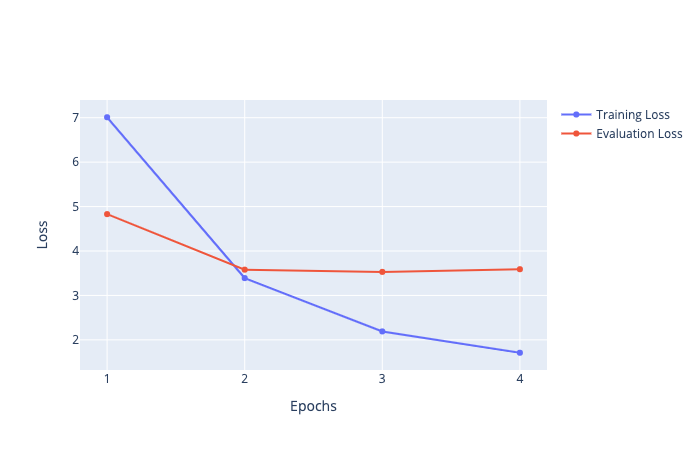
\includegraphics[width=12cm,height=8.5cm]{finetuning_loss.png}\\
  \caption{Training and evaluation loss for finetuning on masked }
  \label{fig:finetuning_loss}
\end{figure}

\begin{figure}[h]
  \centering
  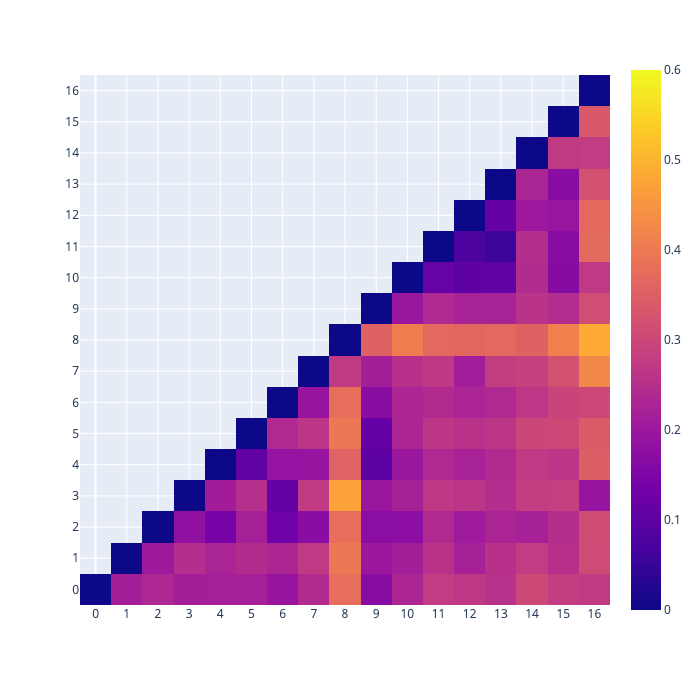
\includegraphics[width=12cm,trim=2cm 2cm .5cm 1cm,clip]{cos_distances_after_clean_with_finetuning.png}\\
  \caption{Cosine distance between templates after cleansing and finetuning}
  \label{fig:cos_distance_finetuning}
\end{figure}


\subsection{Regression}

\section{Discussion of Results}
%TODO box plots of loss values in 